\documentclass[../main.tex]{subfiles}
\graphicspath{{\subfix{../src/}}}


\begin{document}

\section{Methodology}

\subsection{Research Approach}
%\subsection{Introduction of used Software}
%\subsection{Brief of used Software}
\label{sec:software}

In order to design a simulated prosthetic device that facilitates the requirements stated in Section \ref{sec:goals}, effective software solutions needs to be chosen.

A simulation software needs to be chosen in order to create a dynamic and controllable prosthetic hand simulation.
The software needs to be controllable from an external source, in this case ROS2 \cite{ros2}, and because of this, software like Gazebo \cite{gazebo} or CoppeliaSim \cite{coppeliasim} is ideal.
Both simulation software solutions allow for the creation of advanced dynamic-body simulations.
CoppeliaSim \cite{coppeliasim} was chosen due to its intuitive development workflow.

In order to record the joint movements of the hand, while simultaneously record the sEMG activity of the body, products that support hardware synchronization needs to be used.
Products designed to capture sEMG data are widely spread.
As mentioned by Zhaolong Gao et al. \cite{Zhaolong2021}, the myo armband \cite{myo} or the Delsys Trigno package \cite{emgworks} could be used.
The Delsys Trigno \cite{emgworks} facilitates a hardware synchronization recording mode, while the myo armband \cite{myo} does not.
Because of availability, and synchronization capabilities it is ideal to use the Delsys Trigno as the sEMG recording device.

Lastly, a product designed to capture the joint movements of the hand needs to be chosen.
A simple solution to hand tracking would be to use a software like MediaPipe \cite{mediapipe}, a python based landmark tracker that can track the joint angles of the hand using Machine Learning from a video feed.
An alternative is  also mentioned by Zhaolong Gao et al. \cite{Zhaolong2021}, where a glove containing flex sensors could be used.
This approach would provide reliable joint angle data without relying on a camera setup.
Lastly, a capture glove could be fitted with 3D markers, detectable from a high-accuracy and high frame-rate system such as the Motive motion capture setup \cite{optitrack} created by OptiTrack.
It was decided that the the Motive product would be used due to availability and the additional benefit of having a hardware synchronization feature, that can interface with the Delsys Trigno \cite{emgworks} setup.


\subsection{Anatomy of the Lower-Arm}
\label{sec:anatomy}

Dr Arun Pal Singh \cite{anatomy} defines the hand is an anatomically-complex appendage designed to facilitate a large amount of control and adaptability in different usage scenarios.
The hand consists of 27 bones, 14 of these are called the \gls{phalanges}, and make up the 4 fingers and the thumb.
These bones, alongside a complex network of $\sim30$ muscles are able to perform $24$ degree of freedom (DoF) of rotational motion along the joints of the bones.
The individual finger consists of 3 bones called \gls{phalanges}, arranged linearly from the palm of the hand, and can be seen in Figure \ref{fig:anatomy}.
These bones are respectively called the \gls{proximal phalanx}, \gls{middle phalanx} \& \gls{distal phalanx}.
The different joints located in the hand have unique rotation properties.
The joints between the proximal and distal phalanges have 1 DoF of independent movement and are able to do \gls{flexion/extension} movement.
The base of the proximal phalanx has 2 DoF and are able to do \gls{flexion/extension} \& \gls{abduction/adduction} movement.
Additionally, the joint between the middle and distal phalanx is passively moved relative to the proximal and distal phalanx, or in relation to joint constrains from gripped objects.
The wrist consists of 8 small bones and together creates 2 DoF with \gls{flexion/extension} \& \gls{abduction/adduction} movement.

\begin{figure}[H]
\begin{center}
%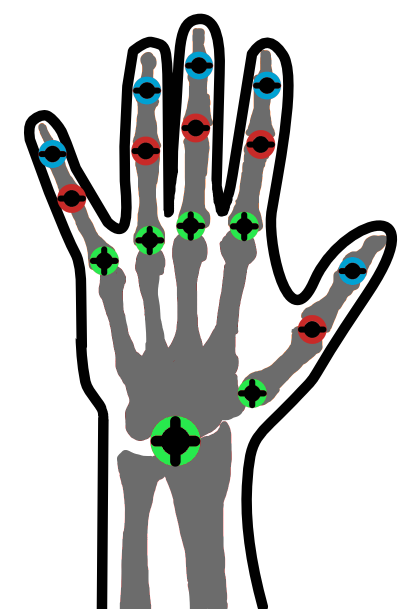
\includegraphics[width=0.6\textwidth, angle=-90]{handjoints.png}
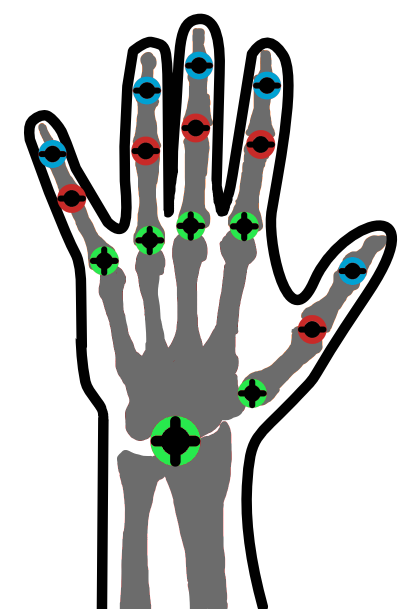
\includegraphics[width=0.5\textwidth]{handjoints.png}
\caption{A rendering of the anatomical joint structure of the hand. 2 DoF joints are colored in green, 1 DoF joints are colored in red, and passive 1 DoF joints are colored in blue.}
\label{fig:anatomy}
\end{center}
\end{figure}

\subsubsection{sEMG Sensor Locations on the Body}
\label{sec:muscleplacements}

To create a dataset that correlates muscle activity to the movements of the hand, it is important to choose a set of active muscles to record.
$\sim 30$ muscles are used in total to control the hand, but it would not be possible to record all of them simultaneously.
6 sEMG sensors were available in the Delsys Trigno \cite{trigno} system, and these needed to be placed optimally in order to increase recording of the most important muscles.
Target areas on the lower-arm for sEMG sensors are proposed by Nestor Jarque-Bou et al. \cite{jarque2019}.
Additionally, target areas of the upper-arm \& upper-body were chosen based on the suggestions from Iason Batzianoulis et al. \cite{Batzianoulis2018}.
The chosen muscles to record with sEMG sensors can be seen in Table \ref{tab:muscletargets}.

\begin{table}[H]
\begin{center}
\begin{tabular}{ |l|l| } 
\hline
Muscle & Main Functionality \\ 
\hline
(A) \textit{Flexor Digitorum Superficialis} & Flexion of the 4 fingers \\
(B) \textit{Extensor Digitorum} & Extension of the fingers \\
(C) \textit{Extensor Carpi Radialis Longus} & Wrist extension \& hand abduction \\
(D) \textit{Triceps Brachii (long head)} & Extension of the arm \\
(E) \textit{Biceps Brachii} & Flexion of the arm \\
(F) \textit{Pectoralis Major + Frontal Deltoid} & Movement of the Arm \\
\hline
\end{tabular}
\caption{The muscles targeted with the 6 available sEMG sensors based on \cite{Batzianoulis2018} \& \cite{jarque2019}.
 The targeted muscles contributes to a lot of the movements of hand \& lower-arm, and are ideal for the dataset.
}
\label{tab:muscletargets}
\end{center}
\end{table}

The target muscles were chosen as they contribute to a lot of the overall movements of the hand \& lower-arm.
The muscles in Table \ref{tab:muscletargets} are numbered, and the locations of the individual sensor with the corresponding muscle can be seen in Figure \ref{fig:musclesensordiagram}.

\begin{figure}[H]
\begin{center}
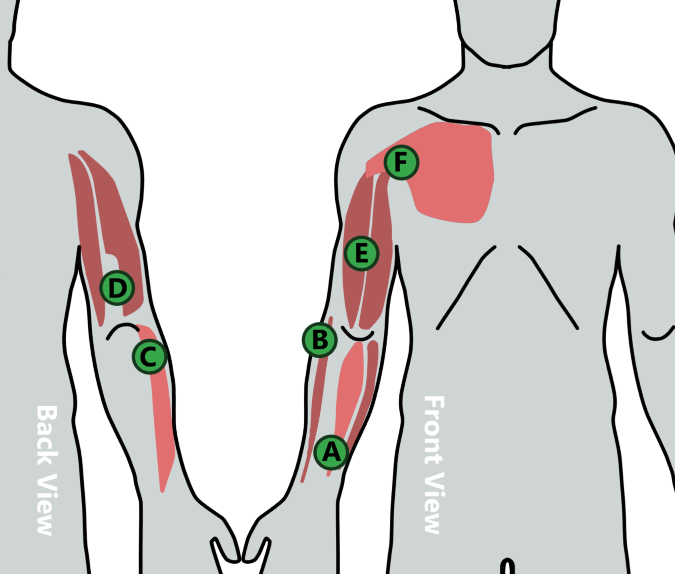
\includegraphics[width=0.8\textwidth]{musclelocations.png}
\caption{Muscle diagram, containing the target sEMG locations. The labeling corresponds to the muscle names in Table \ref{tab:muscletargets}. The left image shows the muscles on the rear of the arm, while the right shows the muscles on the front of the arm.}
\label{fig:musclesensordiagram}
\end{center}
\end{figure}

It was chosen to split the amount of sensors evenly along the lower-arm and the rest of the body in order to asses both direct control of the finger movement and intent based on upper-arm movements.
Alternative muscles that would be interesting to assess are the back muscles, namely \textit{Trapezius} \& \textit{Latissimus Dorsi} as proposed by Keun-Tae Kim et al. \cite{KeunTaeKim2021}.
%how important the different muscles are in prediction of the hand.

\subsection{Design of a Motion Capture Glove}
\label{sec:motiveglove}

The Motive capture system created by OptiTrack \cite{motive} is a set of high quality cameras mounted above a target capture area.
The capture system detects fluorescent 3D markers in the given capture area, with the purpose of triangulating the markers and effectively calculate 3D poses for the markers in the scene down to an effective accuracy of $\pm 0.2$mm.
In order to get precise recordings of the motion of the hand and fingers, fluorescent 3D markers were placed on a glove.
The pattern of the marker positions were chosen in order to calculate the angles of the individual finger bones.
The markers are used in sets of 3, this allows for the calculation of the triangle angles in 3D space.
The positions of the 3D markers on the recorder glove can be seen in Figure \ref{fig:markerdesign} \& \ref{fig:realmarkers}.
An example of \gls{flexion/extension} movement of the capture glove can be seen in Figure \ref{fig:minbend} \& \ref{fig:maxbend}.

%\[
%A = \cos^{-1}\left({\frac{(x_2 - x_1) \cdot (x_3-x_1) +  (y_2 - y_1) \cdot (z_3-z_1)}
%{(\sqrt{(x_2-x_1)^2 +(y_2-y_1)^2 +(z_2-z_1)^2}) \cdot (\sqrt{(x_3-x_1)^2 +(y_3-y_1)^2 +(z_3-z_1)^2}) }}\right)
%\]

\begin{figure}[H]
    \centering
    \begin{subfigure}[b]{0.49\textwidth}
        \centering
        \scalebox{-1}[1]{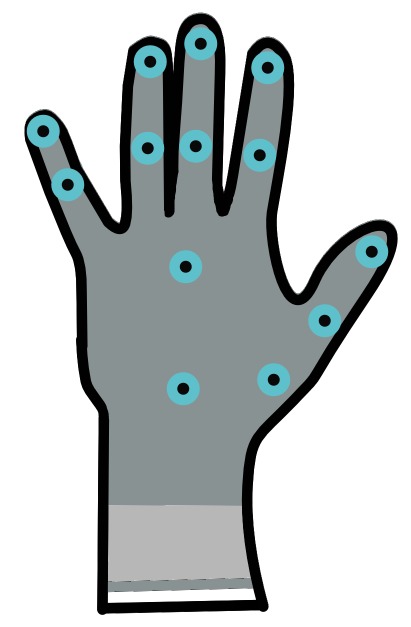
\includegraphics[height=8cm]{glovemarkers.png}}
        \caption{3D marker location design.}
        \label{fig:markerdesign}
    \end{subfigure}
    \hfill
    \centering
    \begin{subfigure}[b]{0.49\textwidth}
        \centering
        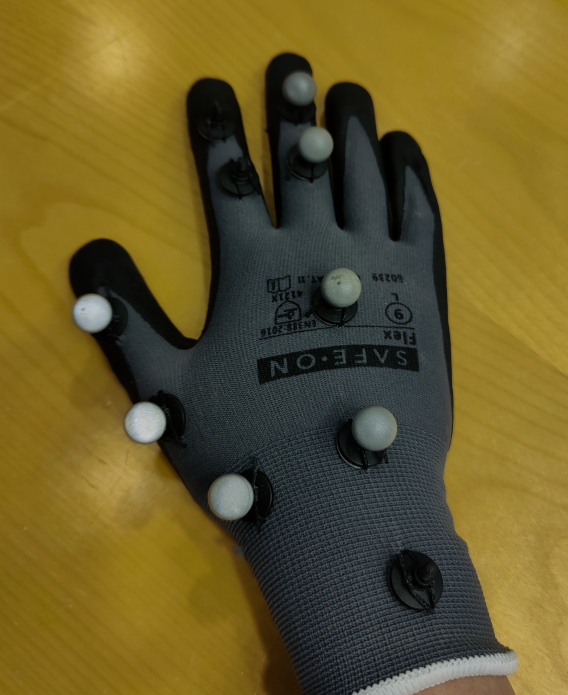
\includegraphics[height=8cm]{realmarkerlocations_cropped.png}
        \caption{Created motion capture glove.}
        \label{fig:realmarkers}
    \end{subfigure}
    \caption{(a) Design and ideal 3D marker placements on the glove in order to calculate all the joint angles of the hand. (b) The created 3D marker glove with the chosen 3D marker locations. See Section \ref{sec:motiveproblems} for detail.}
\end{figure}

Due to the placements of the 3D markers, the joint angles are calculated by defining two vectors from the target 3D marker and using Equation \eqref{eqn:angle}:

\begin{equation}
\label{eqn:angle}
\alpha = \cos^{-1}\left({\frac{\vec{a} \cdot \vec{b}}{ \norm{\vec{a}} \cdot \norm{\vec{b}} }}\right)
\end{equation}


\begin{figure}[H]
    \begin{subfigure}[b]{0.49\textwidth}
        \centering
        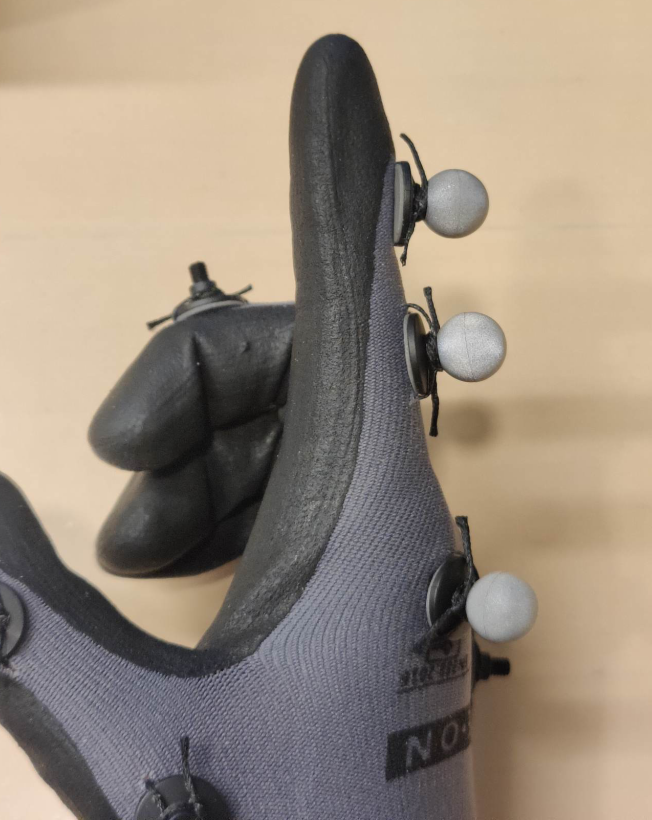
\includegraphics[height=8cm]{motive_glove2_cropped.png}
        \caption{minimum bend of the finger.}
        \label{fig:minbend}
    \end{subfigure}
    \hfill
    \begin{subfigure}[b]{0.49\textwidth}
        \centering
        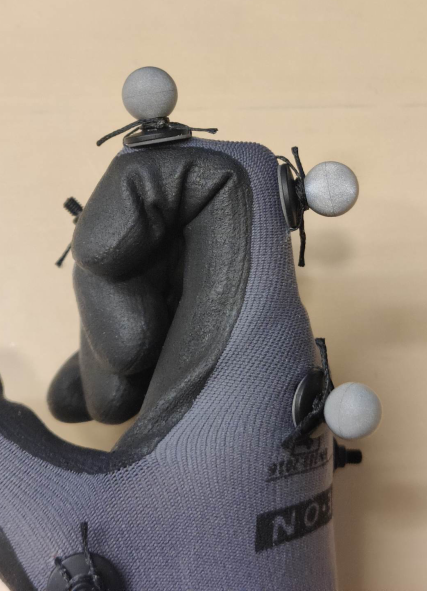
\includegraphics[height=8cm]{motive_glove3_cropped.png}
        \caption{Maximum bend of the finger.}
        \label{fig:maxbend}
    \end{subfigure}
    \caption{Visualization of the joint angle retrieval process. (a) the minimum bend of the \gls{interphalangeal joint}, (b) the maximum bend. The joint angle can be calculated from the 3D markers by denoting vectors from the center marker to upper and lower markers, and using Equation \eqref{eqn:angle}.}

\end{figure}

\subsection{Dataset Creation}
\label{sec:dataset}

In order to create a controller for a prosthetic hand, a sophisticated dataset containing the measured relation between muscle activity and the finger placements is needed.
For such a dataset to represent meaningful data, that can be used to train sophisticated controllers for prosthetic devices, it is important that the dataset is made up of the relevant day-to-day manipulation movements.
%The paper \cite{KeunTaeKim2021} proposes the
\gls{SHAP} \cite{shap} \& ``Sollerman Hand  Function Test''  \cite{sollerman} are applicable procedures of creating a dataset.
Both procedures are used in assessing the function and mobility of the human hand.
By analyzing the most important gripping motions in both tests, it should be possible to denote a suitable set of grips that the dataset needs to contain.
The sollerman grip types are ranked based on their usage percentage in activities of daily living.
From this, the most used grip types according to sollerman are the \textit{Pulp pinch}, \textit{Lateral pinch}, \textit{Five-Finger pinch} \& \textit{Diagonal Volar grip (Power grip)}, see \cite{sollerman} for further details.
SHAP also proposes a set of grip types that are used in day-to-day tasks, these are \textit{Spherical grip}, \textit{Tripod pinch}, \textit{Power grip} \& \textit{Lateral pinch}.
In order to create a dataset mimics the movements of day-to-day tasks, the most important grips from \cite{sollerman} \& \cite{shap} has been chosen.
The grip types that needs to be part of the dataset and their usage descriptions can be seen in Table \ref{tab:grips}.
A set of concise grip types has been chosen as an alternative to a larger set of general grips.
This is done as a basis of creating a specialized dataset that would be easier to train and work with as a proof of concept.
%The chosen grips are chosen as a basis for the creation of a dataset. creating 

\begin{table}[H]
\begin{center}
\begin{tabular}{ |l|l| } 
 \hline
 Grip Type & Object Placement Description \\ 
 \hline
 Pulp pinch & Between thumb, index and middle finger \\ 
 Lateral pinch & Between thumb \& side of index finger \\ 
 Five-Finger pinch & Between thumb, and all four fingers \\ 
 Power grip & Between thumb, and all four fingers with contact to palm \\ 
 \hline
\end{tabular}
\caption{The most used hand grips in day-to-day tasks based on \textit{Southampton Hand Assessment Procedure} \cite{shap} \& \textit{Sollerman Hand Function Test} \cite{sollerman}.}
\label{tab:grips}
\end{center}
\end{table}


\subsubsection{Existing Datasets}

In addition to creating a dataset for this thesis, an existing state-of-the-art dataset is needed.
Nestor Jarque-Bou et al. \cite{jarque2019} proposes the use of their dataset \cite{kinmusdataset}.
The dataset contains a very large set of recordings, with 3 different labeled states, consisting of precise anatomical angles of the hand, with the associated muscle activity of the forearm.
This makes the dataset ideal for both classification and regression based models.
The dataset consists of $572$ recordings from $22$ subjects, in both reaching, gripping \& releasing actions.
Another dataset is referenced by Ashirbad et al. \cite{ashirbad2022}, as an alternative of using finger joint angles as the ground truth data needed to train a network on sEMG data, the dataset uses a set of $16$ gesture classes for a classification algorithm.
%The paper explains that t
The sEMG data in the dataset has been subject to a pre-processing step using a $10$ to $500Hz$ Buttersworth band-pass filter, and a $60Hz$ notch filter was used in order to remove electronics equipment noise.
The dataset was created from recordings of $43$ participants.

\subsubsection{Problems with Motive Tacking Software \& Capture Glove}
\label{sec:motiveproblems}

During testing and the creation of the dataset, several problems with the capture glove design and the capture setup became apparent.
These problem severely reduced the amount of time available to create and process a large dataset for this thesis.
The Motive Motion Capture software \cite{motive} had a lot of difficulty with finding, recording and optimizing the 3D markers placed on the capture glove.

The  Motive software used to generate the 3D poses is designed to detect 3D markers in the scene.
Once the markers are found in the individual cameras, they are subject to an optimization algorithm that effectively tries to determine if the markers seen in 1 camera is the same as the markers in the other cameras.
The first problem that occurred was \gls{specular reflection} in the scene caused by shiny surfaces redirecting light in the target area.
This creates invalid markers that can be seen in only a small set of frames.
Another problem with the capture setup is the optimization algorithm.
During recording of the dataset, it became apparent that it would not be possible to record multiple fingers at the same time.
3D markers very close to each other seemed to be connecting, and only become a single marker in the tracking software.
%Another problem experienced during the creation of a dataset is the dissapearance and merging of markers.
%This problem occurred when two markers had a small distance between them, 
This problem specifically occurred when the markers at the finger tips of the glove came in contact with each other causing marker data to be lost.
Furthermore, the Motive Capture software uses an auto-labeling system that is able to determine if the markers seen in one frame, are the same markers in the next frame.
This system proved to not be reliable, giving $\sim 200$ labeled marker sequences, when only $7$ markers existed in the scene.
%During a sequence of 15 seconds of recording, a set of 7 markers in the scene became over $100$ labeled marker tracks.
The amount of markers increased as 30 seconds of footage became create $\sim 1000$ marker labels.
The problems with the tracking data is assessed in Section \ref{sec:motivecleaning}

\subsection{Design of a Simulated Prosthetic Hand}
\label{sec:prost_sim}

In order to design a state-of-the-art simulated prosthetic hand based on the goals in section \ref{sec:goals}, a number of anatomical design choices needs to be considered.
%This thesis tries to create the most
Designing the simulated prosthetic to as anatomically-correct as possible will hopefully have a number of positive effect on the resulting movement characteristics of the hand, and make it easier to imitate the movements of its real life counterpart.
By having access to an advanced simulation, it is possible to test and visualize advanced movement controllers that can facilitate more DoF than current commercial prosthetic hands. 
By creating an anatomically correct prosthetic hand simulation, it is hoped that prosthesis users can have more advanced rehabilitation, and learn to have more natural control of their prosthetic devices.
Advanced controllers will create a more natural usage experience, and decrease the percentage of users that reject the usage of their prosthetic all together.
A set of requirements the simulated anatomically correct hand should be determined in order to create a state-of-the-art prosthesis simulation.
The simulated prosthetic should:

\begin{enumerate}
\item Facilitate the same DoF as an anatomically correct hand.
\item Have proportions that closely resemble that of an anatomically correct hand.
\item Be simulated and be controllable in a commonly used robotics software to increase accessibility for researchers.
\end{enumerate}

The resulting prosthetic hand simulation can be seen in Appendix \ref{appendix:handsim}.

%\newpage
\subsubsection{Simulated Hand Articulation design}

In order to translate the biology and anatomy of a real hand explained in section \ref{sec:anatomy} into an robotics simulation, the relative lengths of the wrist bones and phalanges were used as reference.
The resulting hand model can be seen in Figure \ref{fig:simdesignandimpl}.
%we start by denoting the relative lengths of the wrist bones and phalnages by refrence, as can be seen in figure \ref{fig:handref}.

\begin{figure}
    \centering
    \begin{subfigure}[b]{0.49\textwidth}
        \centering
        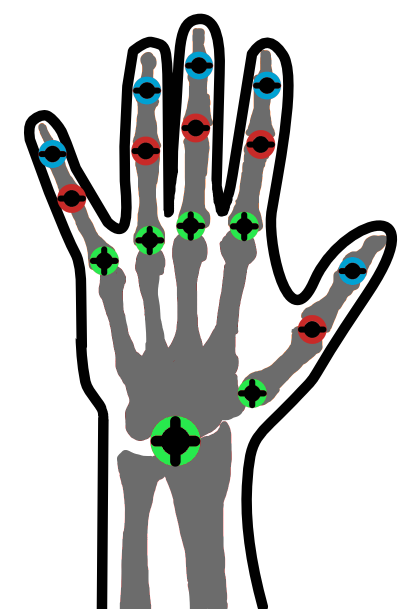
\includegraphics[height=8cm]{handjoints.png}
        %\caption{Created motion capture glove.}
    \end{subfigure}
    \hfill
    \centering
    \begin{subfigure}[b]{0.49\textwidth}
        \centering
        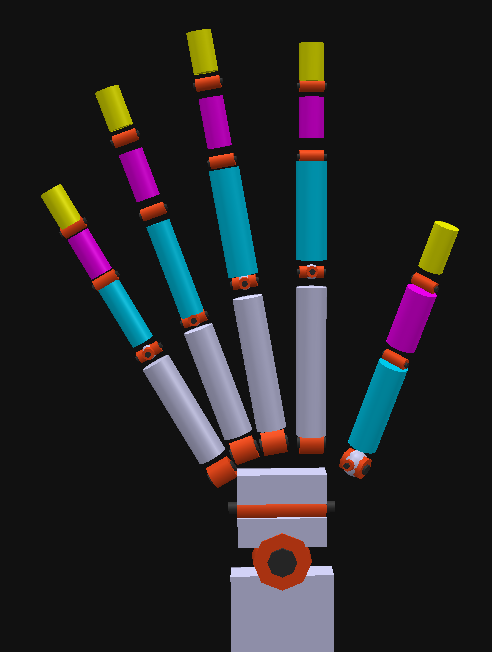
\includegraphics[height=8cm]{simhand.png}
        %\caption{Design of the motion capture glove.}
    \end{subfigure}
    \caption{(Left) Anatomical reference design with placements of different joint types. (Right) The  created simulated prosthetic hand based on the anatomical reference.}
    \label{fig:simdesignandimpl}
\end{figure}

%The porpotions of the refrence is used to denote the bone lengths for the model.
The model is implemented in CoppeliaSim \cite{coppeliasim}, and is based on cylinder shapes of anatomically accurate length and positions,
The phalanges has been colored, with the distal phalanx being yellow, the middle phalanx being purple and the proximal phalanx being blue.
%This colorscheme is chosen in order to make posing clearer.
%The model is created in a hierachy, the bones are created with cylinders and the joints are created using 1 DoF Revolute joints.
% Ref coppeliasim
As specified in section \ref{sec:anatomy}, some joints of the human hand facilitates 2 DoF of rotation.
This is needed in order for the wrist and finger base joints to be able to do \gls{abduction/adduction}.
To simulate this, two 1 DoF revolute joints were placed in series, thus allowing 2 DoF of motion in a single joint.
The resulting simulation can be seen in Appendix \ref{appendix:handsim}.

%\subsection{Software Hand Design}

\end{document}
